\documentclass[11pt]{article}
\usepackage{cite}
\usepackage{color}
\usepackage{authblk}%allows footnote format for authors
\usepackage[letterpaper, margin=1in]{geometry} %package that allows changes in margins and header/footers



\title{Crop adaptation with gene flow from wild relatives}


\author[1] {author1}
\author[1] {author2}
\author[1,2] {author3}
\affil[1]{Department of Ecology, Evolution, and Organismal Biology, Iowa State University, Ames, Iowa, USA}
\affil[2]{Corresponding Author: Matthew B. Hufford; 339A Bessey Hall, Iowa State University, Ames, IA, USA; phone: 1-515-294-8511; email: mhufford@iastate.edu}
\date{}

\begin{document}


\maketitle

\section{Perspectives and key issues}
\begin{itemize}
\item ways to detect gene flow 

compromise between sample size of the source population and the SNP density across the genome
\item ways to detect selection

The methods to detect both gene flow and selection are summarized in Racimo et al. (2015) (archaic adaptive introgression in humans), probably we should not write the first two items.
\item What is the proportion of immigrants showing the signatures of adaptation across the genome
\item Most studies targeted quite long introgression region (in Mb); it is difficult to pinpoint the loci which are introgressed and caused the linkage.
\item The extent to which adapted immigrants are physically linked on chromosomes and reside within structural features restricting recombination, such as inversions
\item the importance of genome structures on local adaptation

An antagonism exists between selection for combination of locally adapted genes, and migration and recombination tending to break them down.
Therefore, genome structures, such as inversion and centromeres, which constrains the recombination, can boost the effectiveness of selection by extending the linkage disequilibrium.
\end{itemize}


\section{Theory of adaptative introgression}

\section{Empirical Data}
\subsection{maize}
Maize is a classical model in crop species to study the issue of adaptive introgresssion from wild relatives, as it is sympatric with a lot of its wild relatives with a range of different divergence time \cite{hufford2013}.
\emph{Zea mays} ssp. \emph{mexicana} (referred to \emph{mexicana} hereafter) and Mexican highland maize is a well-studied pair.
Introgression between \emph{mexicana} and Mexican highland maize has been reported based on evidence from both morphological data \cite {wilkes1977, lauter2004, doebley1984} and molecular analysis \cite{matsuoka2002, vanHeerwaarden2011, doebley1987, warburton2011, fukunaga2005}.
However, \citep{hufford2013} for the first time revealed the evidence of adaptive introgression from \emph{mexicana} to Mexican highland maize.
The authors identified nine genomic regions, which showed evidence of introgression from \emph{mexicana} to maize in both the HAMPMIX and the linkage model of STRUCTURE analyses with over seven sympatric population pairs among the total nine pairs sampled. 
Among the nine regions, three spans the centromeres of chromosomes 5, 6 and 10 and one is located in the inversion polymorphism on chromosome 4, suggesting a significant role of genome structures restricting recombination in adaptive introgression.
By further characterizing the nine introgression regions, it is found that most regions contain long tracts of zero diversity, enriched with QTL linked with anthocyanin content and leaf macrohairs \cite{lauter2004} and over-represented with the SNPs demonstrating high association with temperature seasonality.
It was also revealed that in the growth chamber experiment maize populations with introgression from \emph{mexicana} on chromosome 4 (associated with QTL controlling pigment density and macrohairs) and 9 (overlapped with QTL for macrohairs) exhibited more macrohairs and greater pigmentation under the highland environmental settings than the populations with absence of introgression from \emph{mexicana}.
To put it together, the introgressed alleles/haplotypes from \emph{mexicana} to maize conferred adaptation to highland habitats when maize migrated from Mexican lowlands.
%Finally, the contribution of \emph{mexicana} genetic resource to a broader maize panel was evaluated by analyzing patterns of identity by state (IBS) between maize and \emph{mexicana} as well as between maize and \emph{Zea mays} ssp. \emph {pulviglumis} (referred to \emph {pulviglumis} hereafter).

Even though introgression from \emph{mexicana} to Mexican highland maize has been highly supported \cite{hufford2013}, it is yet unknown whether and to what extent such introgression could be found in other highland maize populations, which are allopatric to \emph{mexicana}. 
A recent study \cite{Takuno2015} found little empirical and theoretical support for parallel highland adaptation in the Mexican and South American highland regions, which was explained partly owing to the difference in the potential for adaptive introgression from wild relatives.
Adaptive SNPs in Mexican highland population were more likely located in the introgressed regions than those in South American highland populations.
Furthermore, the adaptive SNPs in Mexican highland population were more likely also showing signatures of local adaptation in \emph{mexicana} and \emph {pulviglumis} populations than those South American highland population.
To sum up, the adaptive introgression from wild relatives may play a significant role in patterning the genetic differences of maize highland populations.

However, has the introgression from \emph{mexicana} spread to multiple highland populations? 
How does the adaptation differ among populations with and without introgression from \emph{mexicana}?
A recent study \cite{Wang2015manuscript} first utilized the ABBA-BABA statistics to evaluate the existence or absence of introgression from  \emph{mexicana} to multiple highland populations, and then $\hat{f_{d}}$ statistic proposed by Martin et al. (2015) \citep{martin2015} were calculated to locate the introgressed loci. 
Figure \ref{fig:fd} showed the loess regression of $\hat{f_{d}}$ in $10kb$ non\-overlapping windows across two chromosomes (chr4 and chr5) in multiple comparisons. 
On chromosome 4 (Figure \ref{fig:fd}) , Mexican highland (MexHigh) and Guatamalan highland (GuaHigh) exhibited strong evidence of introgression from \emph{mexicana}, and the peaks of distribution corresponded to the region identified in Hufford et al. (2013) \citep{hufford2013}. 
The signal of introgression is absent for the other three populations.
On chromosome 5, the signals of introgression (the peak region of the distribution) are present in MexHigh, GuaHigh and Southwestern US Highland (SW\_US), but not the other two.
More details on the other chromosomes could be referred to \cite{Wang2015manuscript}.
Overall, both analyses revealed that gene flow exist from \emph{mexicana} not only to MexHigh maize, but also to GuaHigh maize, as well as to some individuals in SW\_US, but not to the Andes and South American lowland (SA\_Low) populations, suggesting different extent contributions \emph{mexicana} made to multiple maize highland landrace populations. 
The Andean maize, the population totally isolated from the occurrence of any teosinte species, underwent the severest historical bottleneck, as a population in the front wave of the serial founder effects. 
%The stronger genetic drift introduced by the smaller historical population size improved the homozygosity but reduced the heterozygosity of the population, and it also extended the length of homozygosity.
The high frequency of deleterious alleles caused by stronger genetic drift in the Andes population, together with the reduced efficiency of selection against deleterious sites, contributes to the observed higher mutation load in the well-isolated maize population. 
Even though it is clear that the absence of introgression from wild relatives provided less genetic resource for the highland adaptation and thus made the highland adaptation unique in the Andes, it is yet unknown that out of reach of wild relatives is a reason for reduced fitness in the Andes population.
And the question whether convergent evolution occurs between populations with and without introgression from wild relatives is a key topic for future studies in maize.

\begin{figure*}[b]
\centering
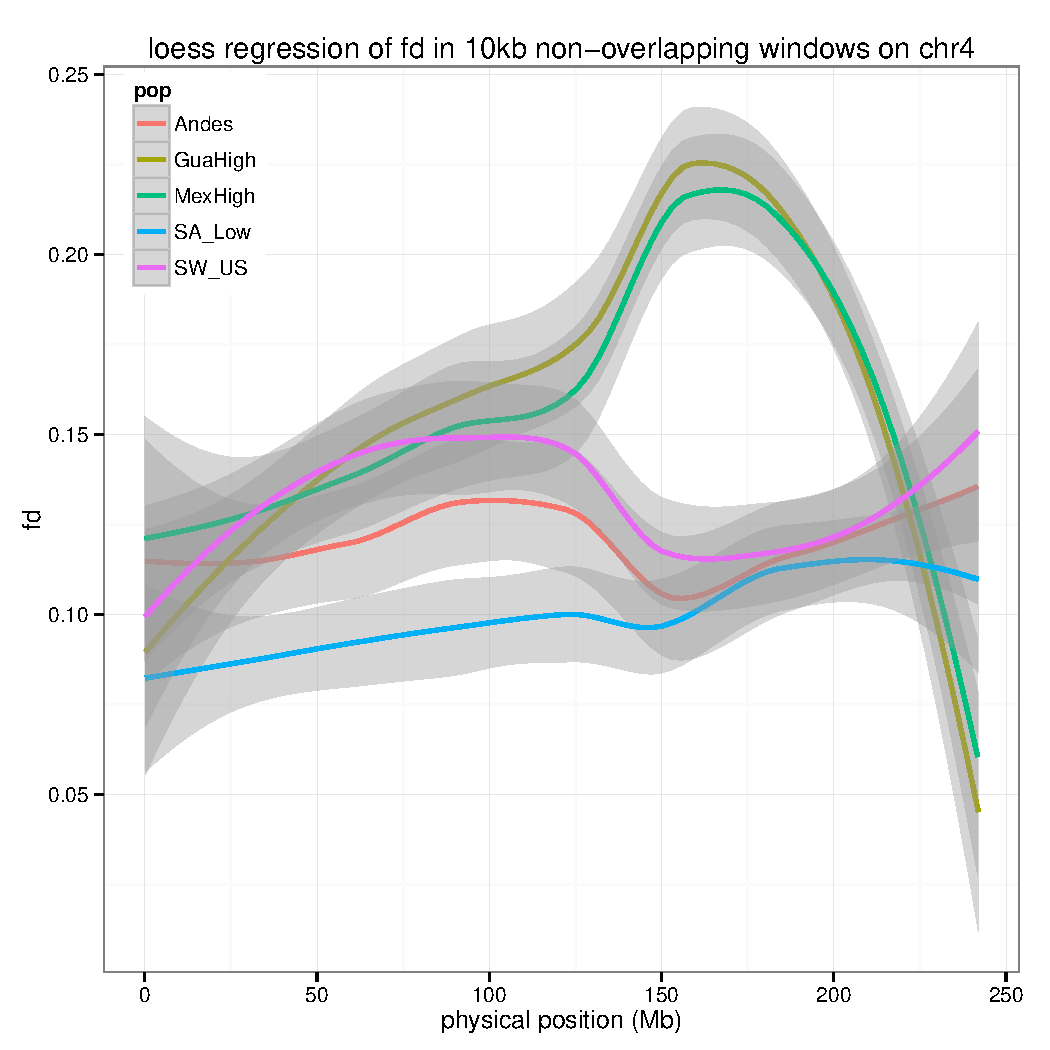
\includegraphics[width=.45\textwidth]{FigsAndTables/fdTrackChr4AllPop}
\hspace{0.05\textwidth} 
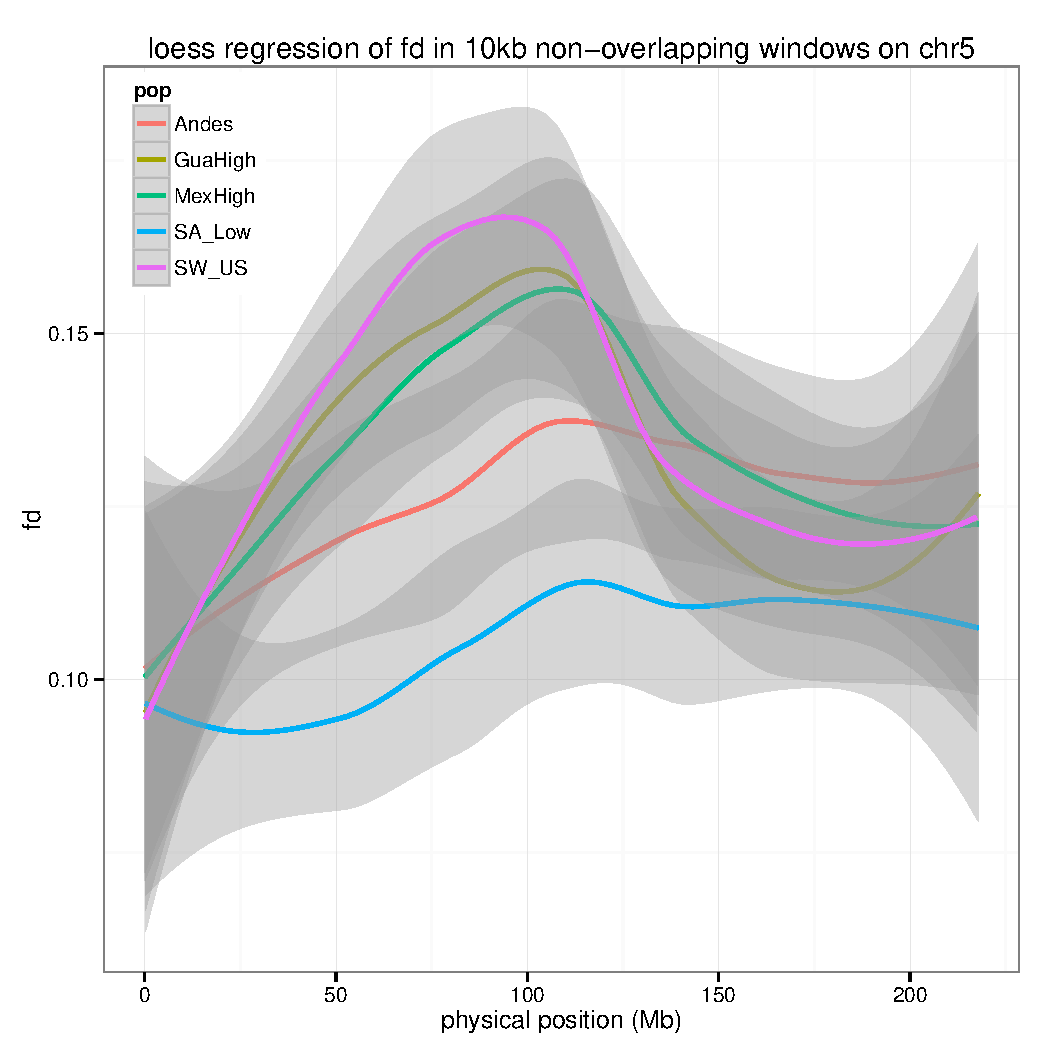
\includegraphics[width=.45\textwidth]{FigsAndTables/fdTrackChr5AllPop}
\caption{Loess regression of $\hat{f_{d}}$ in $10kb$ non\-overlapping windows across the genome in   five independent comparisons: MexLow\-MexHigh\-mexicana\-outgroup, MexLow\-GuaHigh\-mexicana\-outgroup, MexLow\-SW\_US\-mexicana\-outgroup, MexLow\-Andes\-mexicana\-outgroup, MexLow\-SA_Low\-mexicana\-outgroup. A: Chromosome 4; B: Chromosome 5. \label{fig:fd}}
\end{figure*}
 

\subsection{barley}
\subsection{wheat}
\subsection{sunflower}

\section{Concluding remarks and future directions}


\bibliography{Reference}
%\bibliographystyle{...}
%\onecolumn
%\input{supportingInfo} 

% taxa in selection/migration equilibrium
%transition from individual gene to whole-genome understanding
% extent of local adaptation to environmental factors, as well as patterns of gene flow
% migrant alleles or migrant haplotypes





\end{document}
